\chapter{Neutron Production Mechanisms in Liquid Scintillator}\label{chap:yield_theory}

Muons interact with matter through the exchange of virtual photons. The nuclei get excited by the virtual photons, and when they de-excite, neutrons can be released. Neutrons generated by the muon-nucleus interactions are called directly generated neutrons. Electromagnetic fields produced by charged particles can be thought of as a swarm of virtual photons traveling with the particles. When a muon passes by an atomic nucleus, it interacts with the nucleus by exchanging virtual photons with the nucleus. The Feynman diagram for the virtual photon interaction with the nucleus is shown in Figure~\ref{fig:muon_spallation}.
\begin{figure}
	\centering
	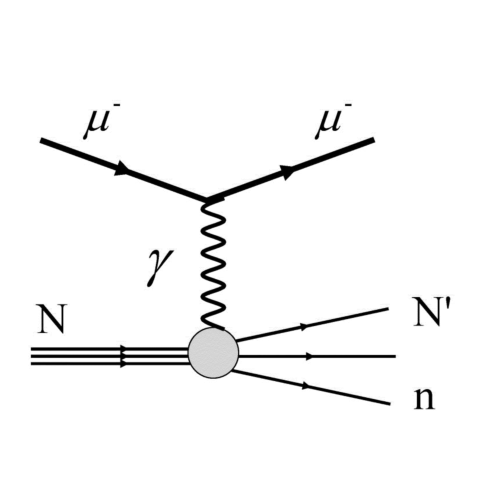
\includegraphics[width=.5\textwidth]{figures/chap6/mu_N_Feynman_diagram.eps}
	\caption{Feynman diagram of muon-nucleus interaction by exchange of a virtual photon.}
	\label{fig:muon_spallation}
\end{figure}
To quantify direct neutron generation, one can first get the virtual photon frequency spectrum with Williams-Weissacker's method of virtual quanta, and then fold it with the photonuclear total cross section of the material under study. The total cross section of the muon-nucleus interaction can then be written as~\cite{Formaggio2004}~\cite{Luu2006}
\begin{equation}\label{eq:mu_N_cross_section}
	\sigma_{\mu N}=\int\frac{n_\gamma(\nu)\sigma_{\gamma N}(\nu)}{\nu}d\nu
\end{equation}
where $n_\gamma(\nu)$ is the virtual photon spectrum associated with the passing muon, $\nu$ is the photon energy, and $\sigma_{\gamma N}(\nu)$ is the real photonuclear cross section. The virtual photon spectrum can be written as~\cite{Delorme1995}
\begin{equation}
	n_\gamma(\nu)=\frac{\alpha}{\pi}\left[\frac{E^2+E'^2}{P^2}\ln\frac{EE'+PP'-m_\mu^2}{m_\mu\nu}-\frac{(E+E')^2}{2P^2}\ln\frac{(P+P')^2}{(E+E')\nu}-\frac{P'}{P}\right]
\end{equation}
where $\alpha$ is the fine structure constant, and $E(E')$ and $P(P')$ are the energy and momentum of the muon before(after) interaction, respectively. The photonuclear cross section was measured by various experiments. Consequently, the cross section of the muon-nucleus interaction can be obtained by Equation~\ref{eq:mu_N_cross_section}. The average number of neutrons $\bar{N}_n$ produced through muon-nucleus interaction by a muon traversing a distance $\ell$ is
\begin{equation}
	\bar{N}_n=n_T\left\langle f\sigma_{\mu N} \right\rangle\ell
\end{equation}
where $n_T$ is the number of target nuclei per unit volume, $f$ is the neutron multiplicity, $\sigma_{\mu N}$ is the muon-nucleus interaction cross section, and $\ell$ is the distance the muon traverses in the medium. The real photon interacts with the nucleus through different mechanisms at different photon energies, and produces a different mean number of neutrons. Thus, when convoluting the virtual photon spectrum with the real photon cross section, different mechanisms have to be considered in accordance with the photon energy. In the order of increasing energy, the dominant processes are giant dipole resonance (GDR) and the $\Delta$ resonance production. Figure~\ref{fig:photo_absorption} shows the photo-absorption cross section of carbon, the dominant element of the liquid scintillator. The peak around 20 MeV corresponds to the GDR and the peak at 300 MeV corresponds to the $\Delta$ production. Figure~\ref{fig:virtual_photon_flux} shows the virtual photon flux $\frac{n_\gamma(\nu)}{\nu}$ for a 100 GeV muon, and Figure~\ref{fig:photonuclear_cross_section} shows the real photonuclear interaction cross section with $^{12}$C from various measurements~\cite{Kossov2002}. Note that $\sigma_{\mu N}$ is the product of the two functions (cf. Figure~\ref{fig:folded_cross_section}), which greatly suppresses the high energy processes due to the deep inelastic scattering.
\begin{figure}
	\centering
	\includegraphics[width=.7\textwidth]{figures/chap6/photo_abroption.png}
	\caption{Solid line shows the photo-absorption cross section of carbon.}
	\label{fig:photo_absorption}
\end{figure}
\begin{figure}
	\centering
  \subfloat[$\frac{n_\gamma(\nu)}{\nu}$]{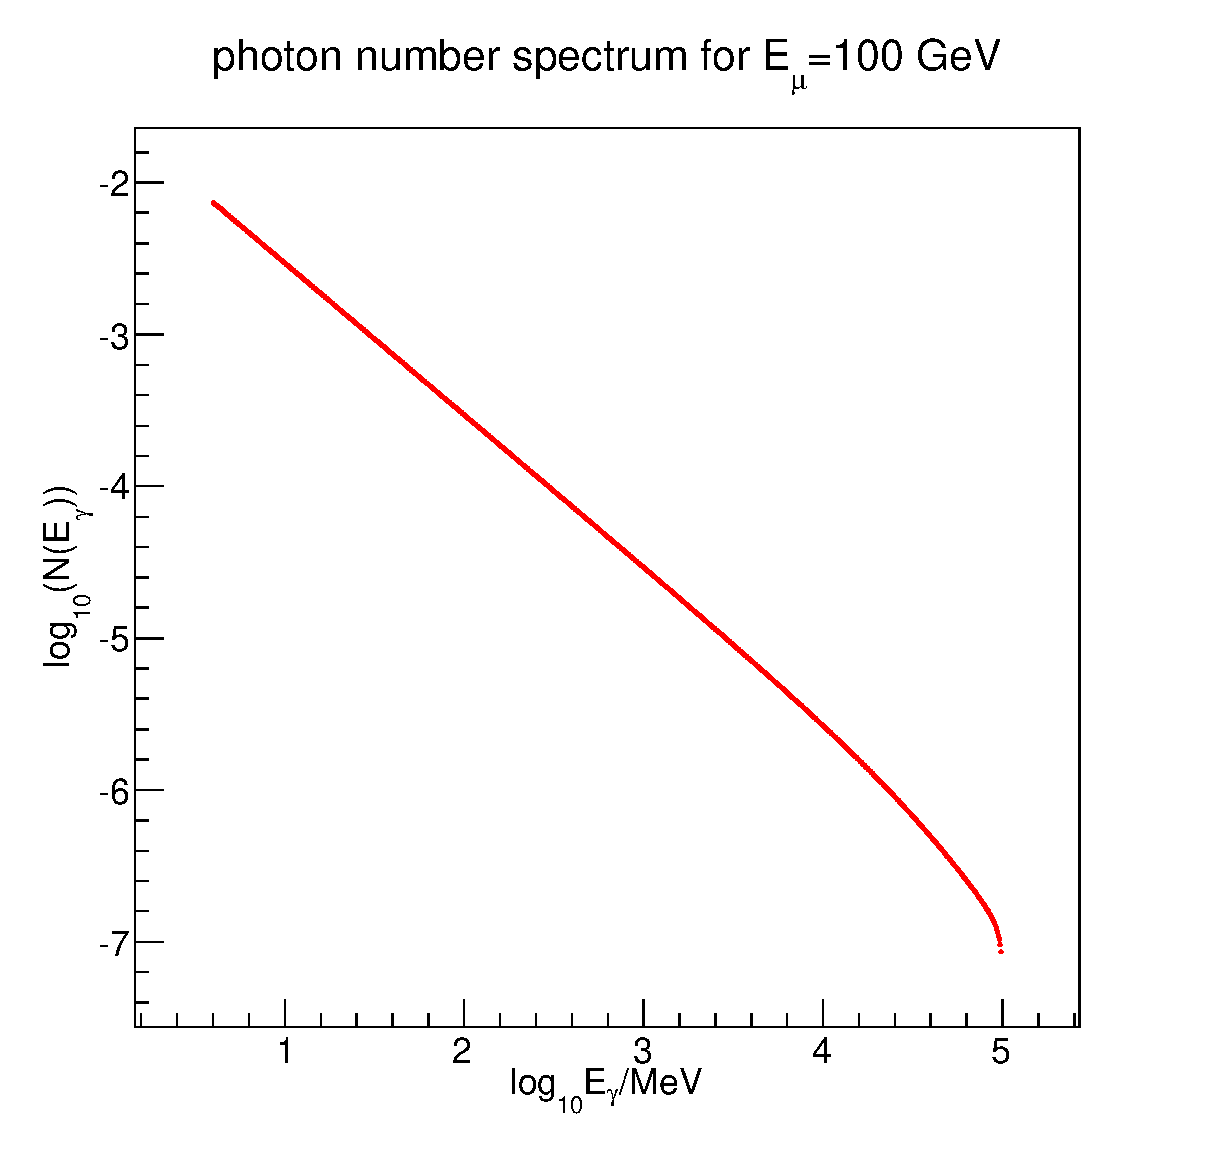
\includegraphics[height=.25\textheight]{figures/chap6/loglog.eps}\label{fig:virtual_photon_flux}}
  \qquad
	\subfloat[photonuclear interaction cross section]{\includegraphics[height=.25\textheight]{figures/chap6/photonuclear.png}\label{fig:photonuclear_cross_section}}
	\caption{The virtual photon flux for a 100 GeV muon and the real photon interaction cross section. The muon nucleus interaction cross section is the product of the two functions.}
\end{figure}

\paragraph{Giant Dipole Resonance}
In the photonuclear interaction cross section, the process taking place with the lowest energy is giant dipole resonance. When photons with wavelength comparable to the size of the nucleus, they see the nucleus as a whole. The oscillating electric field displaces the protons away from their equilibrium position, and an electric dipole is formed. When the giant dipole is formed, the nucleus is in excited state, and when the nucleus de-excites, one or more neutrons can be released. At low photon energies (below $\approx 30$ MeV), photon absorption is dominated by GDR, which decays occasionally by neutron emission~\cite{Bortignon1998}. Table~\ref{table:GDR_carbon}~\cite{IAEALib} shows the threshold energies for different final state particles of the photonuclear reaction with $^{12}$C. This table shows that four decay modes involve at least one neutron in their final states. This indicates the neutron multiplicity of the GDR decay may be larger than one.
\begin{table}
	\centering
	\begin{tabular}{cccccccccc}
	\hline
	Abundance & \multicolumn{9}{c}{Threshold Energies (MeV)} \\
	($\%$) & $\gamma,n$ & $\gamma,p$ & $\gamma,t$ & $\gamma,^3$He & $\gamma,\alpha$ & $\gamma,2n$ & $\gamma,np$ & $\gamma,2p$& $\gamma,3n$ \\
	\hline
	98.89$\%$ & 18.72 & 15.96 & 27.37 & 26.28 & 7.37 & 31.84 & 27.41 & 27.19 & 53.13 \\
	\hline
	\end{tabular}
	\caption{The threshold energies and the released particles for the photonuclear reaction of $^{12}$C.}
	\label{table:GDR_carbon}
\end{table}


%\paragraph{quasideutron}
%With higher photon energy, the photons start to see the proton-neutron pair in the nucleus.


\paragraph{$\Delta$ production}
$\Delta$ resonances are excited states of nucleons. They are a $\pi-N$ state with isospin $I=\frac{3}{2}$ and spin $s=\frac{3}{2}$, where $N$ represents a nucleon. They are the first resonances in $\pi-N$ scatterings. Since resonances decay strongly, they have a typical lifetime of the order of $10^{-23}$ seconds. The properties and decay modes of the $\Delta$ resonances are listed in Table~\ref{table:Delta_resonances}.
\begin{table}
	\centering
	\begin{tabular}{|c|c|c|c|c|c|c|}
	\hline
	particle & quark & \multirow{2}{*}{$I_3$} & \multirow{2}{*}{$J^P$} & \multirow{2}{*}{$Q$} & mean & decay \\
	symbol & content & & & & lifetime (s) & modes \\
	\hline
	$\Delta^{++}(1232)$ & uuu & $\frac{3}{2}$ & $\frac{3}{2}^+$ & +2 & $(5.63\pm 0.14)\times 10^{-24}$ & $\pi^++p$ \\
	\hline
	\multirow{2}{*}{$\Delta^{+}(1232)$} & \multirow{2}{*}{uud} & \multirow{2}{*}{$\frac{1}{2}$} & \multirow{2}{*}{$\frac{3}{2}^+$} & \multirow{2}{*}{+1} & \multirow{2}{*}{$(5.63\pm 0.14)\times 10^{-24}$} & $\pi^0+p$ \\
	& & & & & & $\pi^++n$ \\
	\hline
	\multirow{2}{*}{$\Delta^{0}(1232)$} & \multirow{2}{*}{udd} & \multirow{2}{*}{$-\frac{1}{2}$} & \multirow{2}{*}{$\frac{3}{2}^+$} & \multirow{2}{*}{0} & \multirow{2}{*}{$(5.63\pm 0.14)\times 10^{-24}$} & $\pi^0+n$ \\
	& & & & & & $\pi^-+p$ \\
	\hline
	$\Delta^{-}(1232)$ & ddd & $-\frac{3}{2}$ & $\frac{3}{2}^+$ & -1 & $(5.63\pm 0.14)\times 10^{-24}$ & $\pi^-+n$ \\
	\hline
	\end{tabular}
	\caption{Properties of the $\Delta$ resonances.}
	\label{table:Delta_resonances}
\end{table}
When the photon energy exceeds the pion threshold of 140 MeV, the photons can see individual nucleons. These photons can excite the nucleons and form $\Delta$ resonances. $\Delta$ resonances quickly decay via the strong force into a neutron or a proton and a pion of appropriate charge. The neutrons can leave the nucleus and thus contribute to neutron background. Besides, stopping $\pi^-$'s can form poinic atoms and get captured, producing neutron pairs by the pseudo-deutron capture mechanism $\pi^-+d\rightarrow n+n$.

We can calculate the neutron yield due to this muon-nucleus interaction alone by assuming for each muon-nucleus interaction, one neutron is released. Then the neutron yield can be linked to the total cross section of the muon-nucleus interaction by the following formula,
\begin{equation}
	Y_n=\frac{P}{\ell \rho}=\sigma n=\frac{\sigma N_A}{A}
\end{equation}
where $Y_n$ is the neutron yield, $P$ is the interaction probability, $\ell$ is the track length, $\rho$ is the material density, $n$ is the number density, $N_A$ is the Avogadro's number, and $A$ is the atomic mass of the material. Since muons with different energies have different virtual photon energy spectra, here we use the mean muon energy typical of all Daya Bay's experimental halls as the muon energy, i.e. 100 GeV. The blue curve in Figure~\ref{fig:folded_cross_section} shows the product of the virtual photon energy spectrum and the real photonuclear cross section shown in Figure~\ref{fig:virtual_photon_flux}. The red curve in Figure~\ref{fig:folded_cross_section} is the cumulative integral of the blue curve.
\begin{figure}
	\centering
	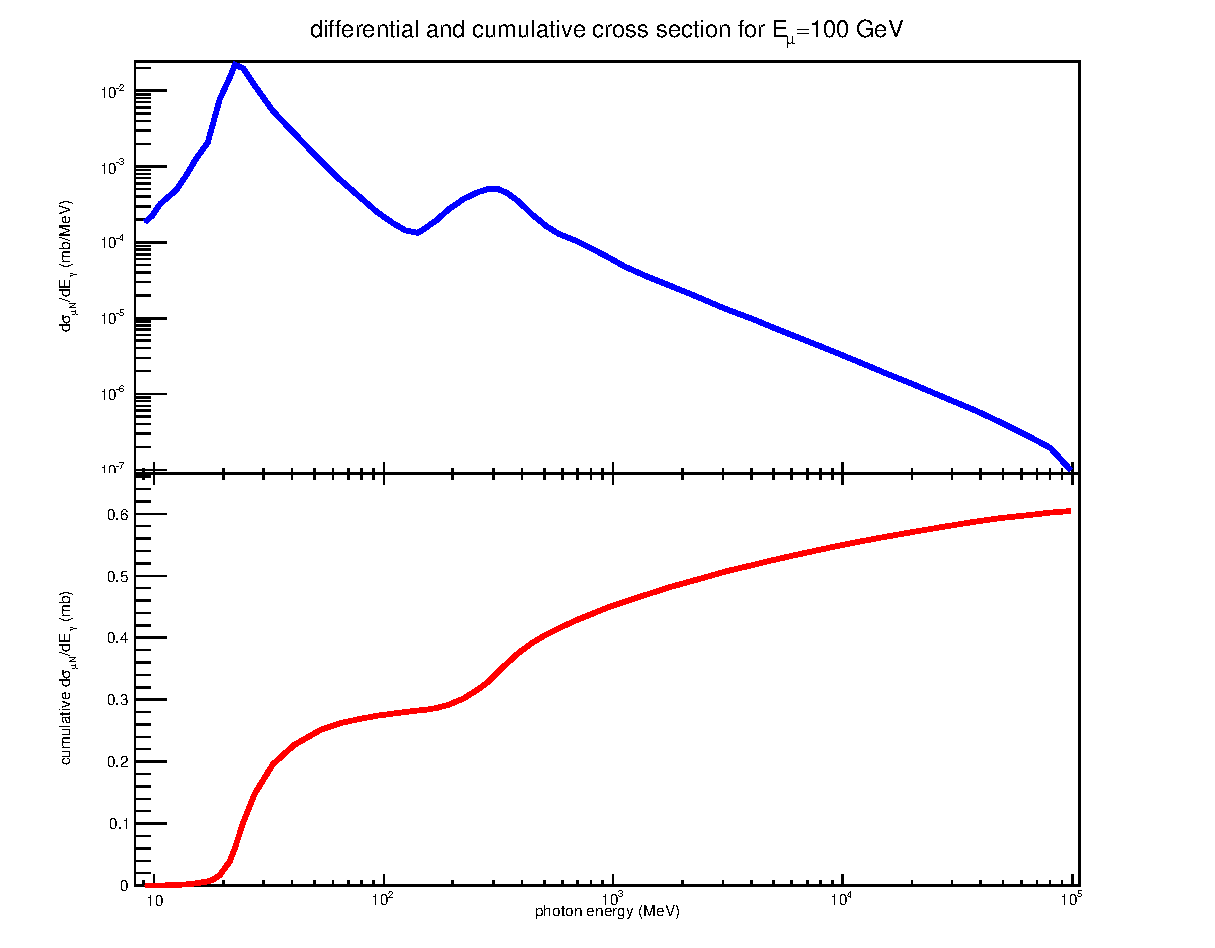
\includegraphics[width=.8\textwidth]{figures/chap6/muN_diff_cumul_cross_section.eps}
	\caption{Top: Muon nucleus differential cross section for 100 GeV muons. Bottom: Cumulative muon nucleus cross section for 100 GeV muons.}
	\label{fig:folded_cross_section}
\end{figure}
The integral of the differential cross section over all photon energy gives the total cross section $\sigma=0.6$ mb. Therefore the neutron yield is
\begin{equation}
	Y_n=\frac{0.6(mb)\times 10^{-27}\left(\frac{cm^2}{mb}\right)\times 6.02\times10^{23}\left(\frac{1}{mol}\right)}{12\left(\frac{g}{mol}\right)}=3\times 10^{-5} (cm^2/g)
\end{equation}
The cumulative cross section shows that the GDR contribution to the total cross section is roughly the same as the contribution from $\Delta$ production and higher energy processes. The yield calculated this way is in rough agreement with the data to be presented in Chapter~\ref{chap:results}. The discrepancy is probably due to higher neutron multiplicity, secondary interactions, and residual high energy interactions.